\input{src/header}											% bindet Header ein (WICHTIG)
\usepackage{graphicx}

\newcommand{\dozent}{Prof. Dr. Margarita Esponda}					% <-- Names des Dozenten eintragen
\newcommand{\tutor}{Lilli Walter}						% <-- Name eurer Tutoriun eintragen
\newcommand{\tutoriumNo}{Tutorium 6}				% <-- Nummer im KVV nachschauen
\newcommand{\projectNo}{1}									% <-- Nummer des Übungszettels
\newcommand{\veranstaltung}{Nichtsequentielle Programmierung}	% <-- Name der Lehrveranstaltung eintragen
\newcommand{\semester}{SoeSe 2017}						% <-- z.B. SoSo 17, WiSe 17/18
\newcommand{\studenten}{Boyan Hristov}			% <-- Hier eure Namen eintragen
% /////////////////////// BEGIN DOKUMENT /////////////////////////


\begin{document}
% /////////////////////// BEGIN TITLEPAGE /////////////////////////
\begin{titlepage}
	\subject{\dozent}
	\title{\veranstaltung, \semester}
	\subtitle{\Large Übungsblatt \projectNo\\ \large\vspace{1ex} }
	\author{\studenten}
	\date{\normalsize \today}
\end{titlepage}

\maketitle								% Erstellt das Titelblatt
\vspace*{-9cm}							% rückt Logo an den oberen Seitenrand
\makebox[\dimexpr\textwidth+1cm][r]{	%rechtsbündig und geht rechts 1cm über Layout hinaus
	\includegraphics[width=0.4\textwidth]{src/fu_logo} % fügt FU-Logo ein
}
% /////////////////////// END TITLEPAGE /////////////////////////

\vspace{7cm}							% Abstand
\rule{\linewidth}{0.8pt}				% horizontale Linie										% erstellt die Titelseite


% /////////////////////// Aufgabe 1 /////////////////////////
\section{Aufgabe}
Man kann erkenne, dass Wechselseitige Ausschluss gewährleistet ist, da es keine Zustände (p3, r3) für den 1. Algorithmus und (p5, r5) für den 2. Algorithmus existieren.

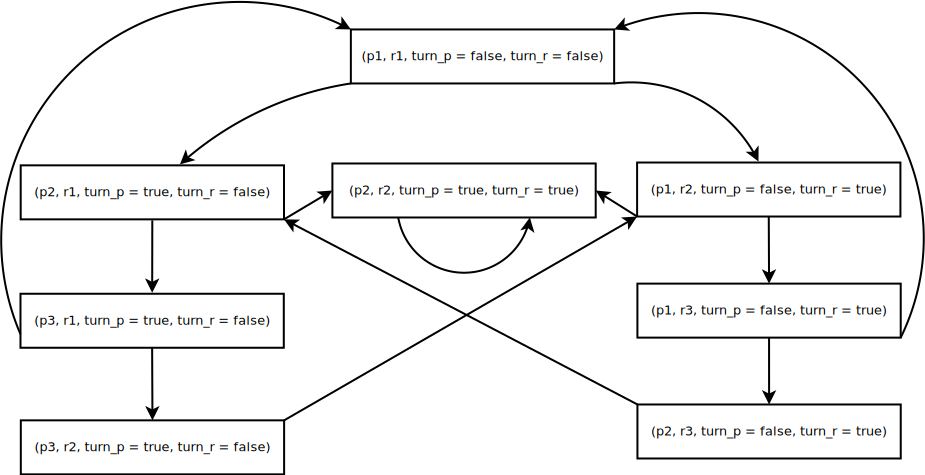
\includegraphics[width=\textwidth]{./exercise1/diagramm-1-A.png}

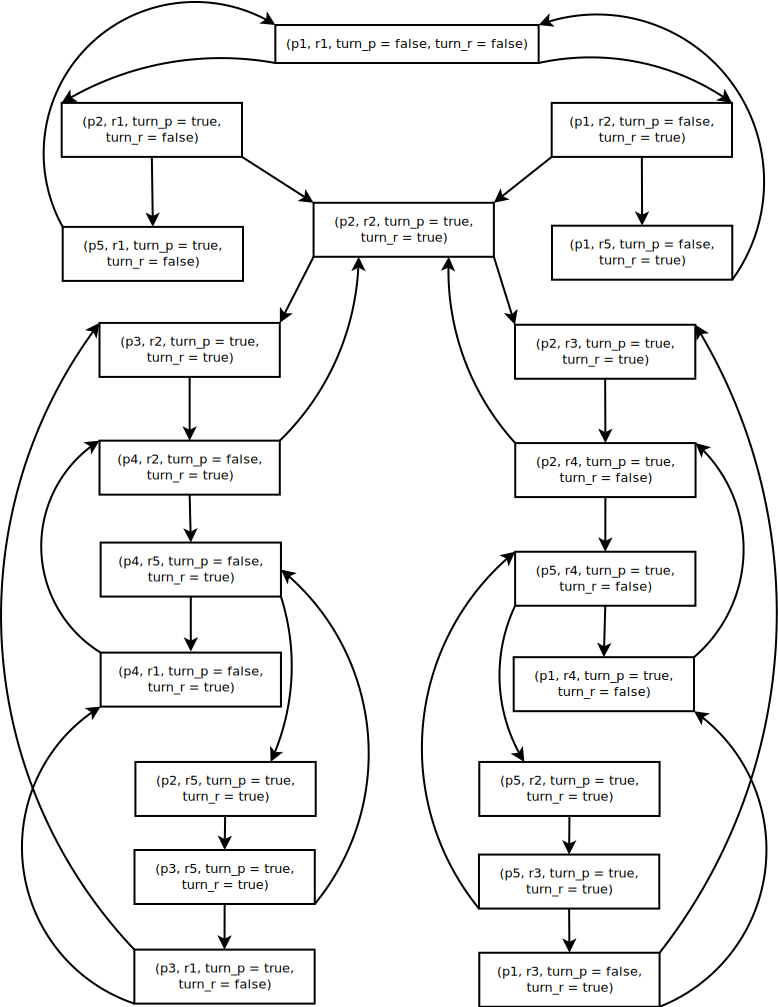
\includegraphics[width=\textwidth]{./exercise1/diagramm-1-B.png}

% /////////////////////// Aufgabe 2 /////////////////////////
\section{Aufgabe}

Wir haben irgendwann erkannt, dass die Idee die Aufgabe nicht solche ist, da diese nur 8 Punkte gibt. Eigentlich ist aber in Assembler so, dass man erstmal ein Exchange machen kann, und dann noch Compare + JE oder JNE. Wir haben deswegen gemeint, dass 'until !local\_r' eine Art von 'If true, jump to r2/p2, else continue to r4/p4'. Wir dachten dass es trotzdem Sinn macht diese Variante zu zeigen, wollten auch unsere Arbeit nicht wegschmeißen. \\

Man erkennt, dass es keine Deadlocks gibt, da es keine Zustände gibt mit nur eingehende Pfeile. 
Wechselseitige Ausschluss ist auch gewährleistet, da die verbotene Zustände (diese, die p4 und r4 gleichzeitig enthalten) nicht existieren.

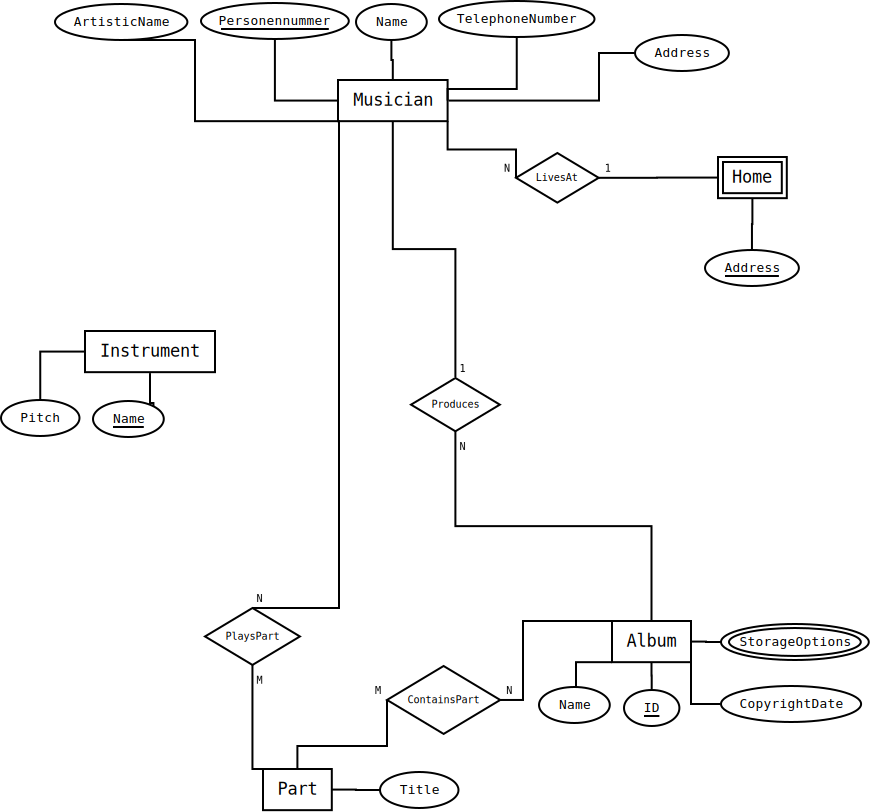
\includegraphics[width=\textwidth]{./exercise2/exercise2.png}

\section{Aufgabe}





% /////////////////////// END DOKUMENT /////////////////////////
\end{document}